\documentclass[10pt,]{article}
\usepackage[left=1in,top=1in,right=1in,bottom=1in]{geometry}
\newcommand*{\authorfont}{\fontfamily{phv}\selectfont}
\usepackage[]{mathpazo}


  \usepackage[T1]{fontenc}
  \usepackage[utf8]{inputenc}



\usepackage{abstract}
\renewcommand{\abstractname}{}    % clear the title
\renewcommand{\absnamepos}{empty} % originally center

\renewenvironment{abstract}
 {{%
    \setlength{\leftmargin}{0mm}
    \setlength{\rightmargin}{\leftmargin}%
  }%
  \relax}
 {\endlist}

\makeatletter
\def\@maketitle{%
  \newpage
%  \null
%  \vskip 2em%
%  \begin{center}%
  \let \footnote \thanks
    {\fontsize{18}{20}\selectfont\raggedright  \setlength{\parindent}{0pt} \@title \par}%
}
%\fi
\makeatother




\setcounter{secnumdepth}{0}


\usepackage{graphicx}
% We will generate all images so they have a width \maxwidth. This means
% that they will get their normal width if they fit onto the page, but
% are scaled down if they would overflow the margins.
\makeatletter
\def\maxwidth{\ifdim\Gin@nat@width>\linewidth\linewidth
\else\Gin@nat@width\fi}
\makeatother
\let\Oldincludegraphics\includegraphics
\renewcommand{\includegraphics}[1]{\Oldincludegraphics[width=\maxwidth]{#1}}

\title{Assesing Health Care Coverage and Access Utilizing the National Health
Interview Survey  }



\author{\Large John Diego\vspace{0.05in} \newline\normalsize\emph{University of Washington}   \and \Large Warren Wakuzawa\vspace{0.05in} \newline\normalsize\emph{University of Washington}   \and \Large Adrian Santiago\vspace{0.05in} \newline\normalsize\emph{University of Washington}  }


\date{}

\usepackage{titlesec}

\titleformat*{\section}{\normalsize\bfseries}
\titleformat*{\subsection}{\normalsize\itshape}
\titleformat*{\subsubsection}{\normalsize\itshape}
\titleformat*{\paragraph}{\normalsize\itshape}
\titleformat*{\subparagraph}{\normalsize\itshape}





\newtheorem{hypothesis}{Hypothesis}
\usepackage{setspace}

\makeatletter
\@ifpackageloaded{hyperref}{}{%
\ifxetex
  \usepackage[setpagesize=false, % page size defined by xetex
              unicode=false, % unicode breaks when used with xetex
              xetex]{hyperref}
\else
  \usepackage[unicode=true]{hyperref}
\fi
}
\@ifpackageloaded{color}{
    \PassOptionsToPackage{usenames,dvipsnames}{color}
}{%
    \usepackage[usenames,dvipsnames]{color}
}
\makeatother
\hypersetup{breaklinks=true,
            bookmarks=true,
            pdfauthor={John Diego (University of Washington) and Warren Wakuzawa (University of Washington) and Adrian Santiago (University of Washington)},
             pdfkeywords = {healthcare, NHIS, ACA, medicaid, medicare},  
            pdftitle={Assesing Health Care Coverage and Access Utilizing the National Health
Interview Survey},
            colorlinks=true,
            citecolor=blue,
            urlcolor=blue,
            linkcolor=magenta,
            pdfborder={0 0 0}}
\urlstyle{same}  % don't use monospace font for urls



\begin{document}
	
% \pagenumbering{arabic}% resets `page` counter to 1 
%
% \maketitle

{% \usefont{T1}{pnc}{m}{n}
\setlength{\parindent}{0pt}
\thispagestyle{plain}
{\fontsize{18}{20}\selectfont\raggedright 
\maketitle  % title \par  

}

{
   \vskip 13.5pt\relax \normalsize\fontsize{11}{12} 
\textbf{\authorfont John Diego} \hskip 15pt \emph{\small University of Washington}   \par \textbf{\authorfont Warren Wakuzawa} \hskip 15pt \emph{\small University of Washington}   \par \textbf{\authorfont Adrian Santiago} \hskip 15pt \emph{\small University of Washington}   

}

}







\begin{abstract}

    \hbox{\vrule height .2pt width 39.14pc}

    \vskip 8.5pt % \small 

\noindent The National Health Interview Survey (NHIS) is the nation's largest
in-person household health survey. It has been conducted annually since
1957 by the National Center for Health Statistics (NCHS), which is a
part of the Centers for Disease Control and Prevention (CDC). A broad
range of topics are covered but we will specifically focus on healthcare
access and expenditure across a multitude of factors such as employer
information, race, and academic background.


\vskip 8.5pt \noindent \emph{Keywords}: healthcare, NHIS, ACA, medicaid, medicare \par

    \hbox{\vrule height .2pt width 39.14pc}



\end{abstract}


\vskip 6.5pt

\noindent  \section{INTRODUCTION}\label{introduction}

The Patient Protection and Affordable Care Act (PPACA), commonly
shortened to the Affordable Care Act (ACA) and nicknamed Obamacare, is
one of the most important healthcare legislature, creating a significant
impact on the US Health care system. However, with the arrival of
President Trump in the Oval Office, and with the ACA repeal now
underway, some speculate huge consequences such as
\href{https://www.washingtonpost.com/posteverything/wp/2017/01/23/repealing-the-affordable-care-act-will-kill-more-than-43000-people-annually/?utm_term=.a2fbb24cd075}{increased
death rates}. In light of these recent events, it is important that we
take a look at the current state of our healthcare system and question
whether it is failing or not.

The purpose of this paper is to assess healthcare coverage and access
across a multitude of factors. We will specifically look at three
aspects of health care - the first aspect is the relationship between
educational attainment and access to medical insurance, the second is an
overall look at the population and health care coverage, and the final
exploration covers healthcare expenditure over the years.

\section{METHODOLOGY}\label{methodology}

To answer the questions we layed out, we use data provided from the NHIS
survey. We used various subsets of the survey data, depending on the
specific question being analyzed.

\subsection{\texorpdfstring{\textbf{Educational Attainment Vs Healthcare
Access}}{Educational Attainment Vs Healthcare Access}}\label{educational-attainment-vs-healthcare-access}

\subsection{\texorpdfstring{\textbf{Health Care
Access}}{Health Care Access}}\label{health-care-access}

\subsection{\texorpdfstring{\textbf{Health Care
Expedentiture}}{Health Care Expedentiture}}\label{health-care-expedentiture}

To gain a general outlook on the healthcare system, one way of looking
at it is through the perspective of expenditures. Specifically the
question we wanted to explore is, \emph{``How has the amount of money
spent for medical care changed over the years?''} One specific variable
that was counted for from the survey was \emph{``Amount family spent for
medical care, past 12 months''}. To see this distribution, data from the
2005 to 2015 NHIS surveys was used (N=1,033,155). We then filtered the
data further down to those who responded back to the question (N =
994,797). The distribution of health expenditure over the years can be
seen in the graph below.

This independent variable only provides a rough estimate on the family's
expenditure on medical care, but is still relevant since interviewers
directed respondents to exclude the insurance premiums, over-the-counter
drugs, and any costs for which they expected to be reimbursed.

To make calculations on the greater population, we used the calculated
weight and strata within the provided by those who constructed the NHIS
dataset. According to the \href{https://ihis.ipums.org/}{codebook}, the
\emph{sample weight} was calculated using ``adjustments for age,
race/ethnicity, and sex using the Census Bureau's population control
totals'', while \emph{strata} was represents ``the impact of the sample
design stratification on the estimates of variance and standard
errors.'' A \textbf{stratified random sampling} was implemented to
calculate the weighted proportions of people who spend X amount for
health insurance, X being multiple levels of range of money spent.

\section{RESULTS}\label{results}

\subsection{\texorpdfstring{\textbf{Plots}}{Plots}}\label{plots}

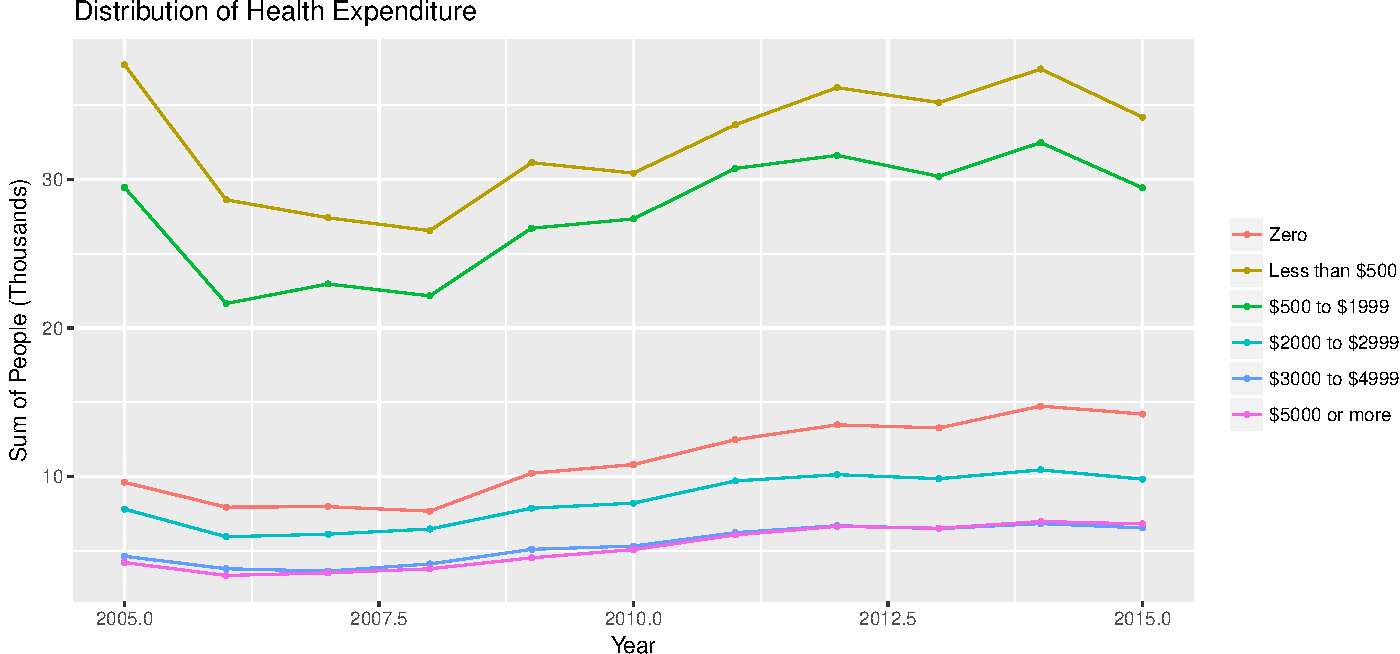
\includegraphics{paper_files/figure-latex/expenddistribution-1.pdf}
\textbf{Figure 1. Expenditure Distribution over Time}

\smallskip

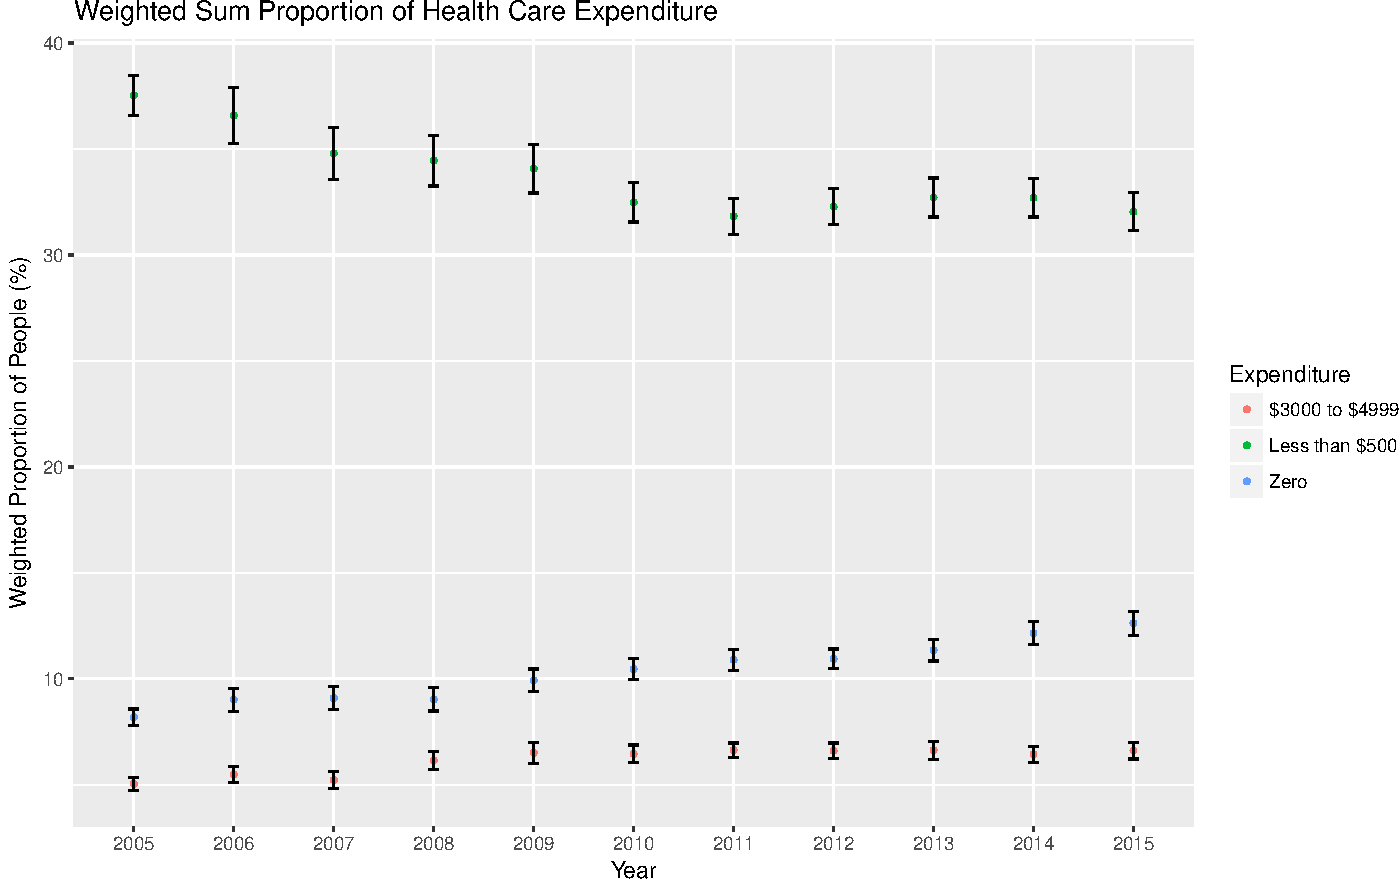
\includegraphics{paper_files/figure-latex/weightedexpendproportion-1.pdf}
\textbf{Figure 2. Expenditure Distribution over Time (Weighted)}

\smallskip

\section{DISCUSSION}\label{discussion}

\subsection{\texorpdfstring{\textbf{Educational Attainment Vs Healthcare
Access}}{Educational Attainment Vs Healthcare Access}}\label{educational-attainment-vs-healthcare-access-1}

\subsection{\texorpdfstring{\textbf{Health Care
Access}}{Health Care Access}}\label{health-care-access-1}

\subsection{\texorpdfstring{\textbf{Health Care
Expedentiture}}{Health Care Expedentiture}}\label{health-care-expedentiture-1}

For the chart concerning health care expenditure (Figure 2), We can see
the proportion of people who spent a specific level of money on health
insurance, whether it be zero,less than 500\$, or the other levels. For
example, we see that the largest proportion of people mostly spent less
than 500 dollars through out time, with atleast more than 30\% given any
year. Specifically, for 2005, 37.5\% percent of the population
\emph{spent less than 500 dollars}, but for 2015, it went down to
32.04\%. For the people \emph{spending no money} on health insurance,
this proportion mostly stayed between 8\% to 12\% over the years, with a
positive increase over time. Meanwhile, The proportion of people
\emph{spending between 3000 to 4000 dollars} doesn't have a linear
change over time like the other levels of expedenture. This proportion
stayed between 5\% and 6\% over time. Showing no linear change for
\emph{spending between 3000 to 4000 dollars} can be interpreted as a
positive income, since that means the proportion of the population
spending money on health insurance are not seeing an increase of
expenditure. One would expect that with the introduction of the
Affordable Care Act in 2010, which promised reducing health care costs,
the amount of money people are spending on health care would decrease.
These expectations turned out to be true, since the graph reflects a
positive rate of change for people spending no money on health
insurance, and negative rate of change for people spending less than 500
dollars.

\section{RELATED WORK}\label{related-work}

A description of previous papers or projects related to your project.

\section{CONLUSION}\label{conlusion}

Final summary and a description of how your system could be extended.

\section{REFERENCES}\label{references}

\begin{enumerate}
\def\labelenumi{\arabic{enumi}.}
\item
  IPUMS Health Surveys. Retrieved February 27, 2017 from
  \url{https://ihis.ipums.org/ihis/index.shtml}
\item
  David Himmelstein,Steffie Woolhandler. January 23, 2017. Repealing the
  Affordable Care Act will kill more than 43,000 people annually.
  Retrieved March 6, 2017 from
  \url{https://www.washingtonpost.com/posteverything/wp/2017/01/23/repealing-the-affordable-care-act-will-kill-more-than-43000-people-annually/?utm_term}=.a2fbb24cd075
\end{enumerate}
\newpage
\singlespacing 
\end{document}svm